
%(BEGIN_QUESTION)
% Copyright 2006, Tony R. Kuphaldt, released under the Creative Commons Attribution License (v 1.0)
% This means you may do almost anything with this work of mine, so long as you give me proper credit

Se på følgende fireelektrode-krets for ledningsevneanalyse, og svar på spørsmålene:

$$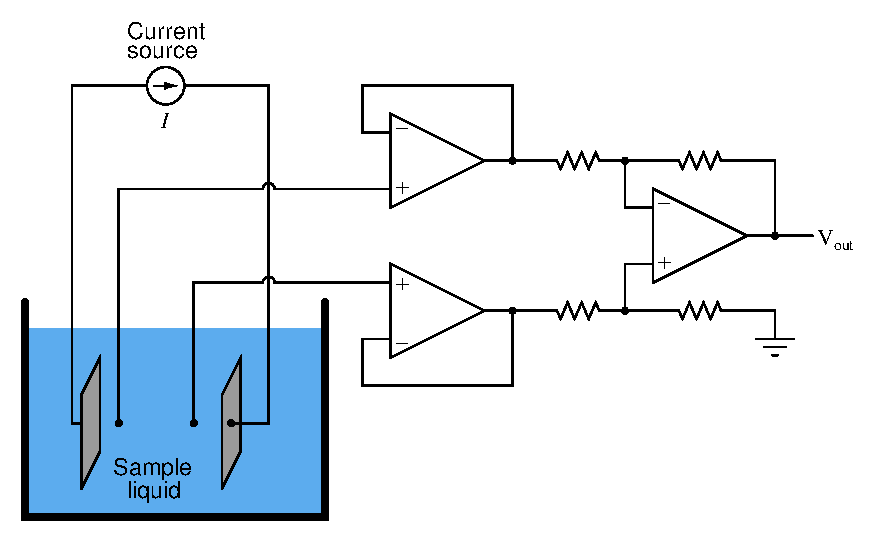
\includegraphics[width=15.5cm]{i00910x01.eps}$$

\begin{itemize}
\item{} Hvis strømkildens utgang øker, vil $V_{out}$ {\it øke}, {\it minke}, eller {\it være uendret}?
\vskip 5pt
\item{} Hvis ledningsevnen i væsken øker, vil $V_{out}$ {\it øke}, {\it minke}, eller {\it være uendret}?
\vskip 5pt
\item{} Hvis de to ytre elektrodene (koblet til strømkilden) får belegg av mineraler eller annet ikke-ledende materiale, vil $V_{out}$ {\it øke}, {\it minke}, eller {\it være uendret}?
\vskip 5pt
\item{} Hvis prøvevæsken er springvann, nevn noe du kan gjøre med vannet for å øke ledningsevnen.
\end{itemize}

\underbar{file i00910}
%(END_QUESTION)





%(BEGIN_ANSWER)

\begin{itemize}
\item{} Hvis strømkildens utgang øker, vil $V_{out}$ {\bf øke}.
\vskip 5pt
\item{} Hvis ledningsevnen i væsken øker, vil $V_{out}$ {\bf minke}.
\vskip 5pt
\item{} Hvis de to ytre elektrodene (koblet til strømkilden) får belegg av mineraler eller annet ikke-ledende materiale, vil $V_{out}$ {\bf være uendret}.
\vskip 5pt
\item{} Du kan tilsette salt eller en annen ionisk forbindelse i vannet for å øke ledningsevnen. Du kan også varme opp vannet.
\end{itemize}

%(END_ANSWER)





%(BEGIN_NOTES)

$$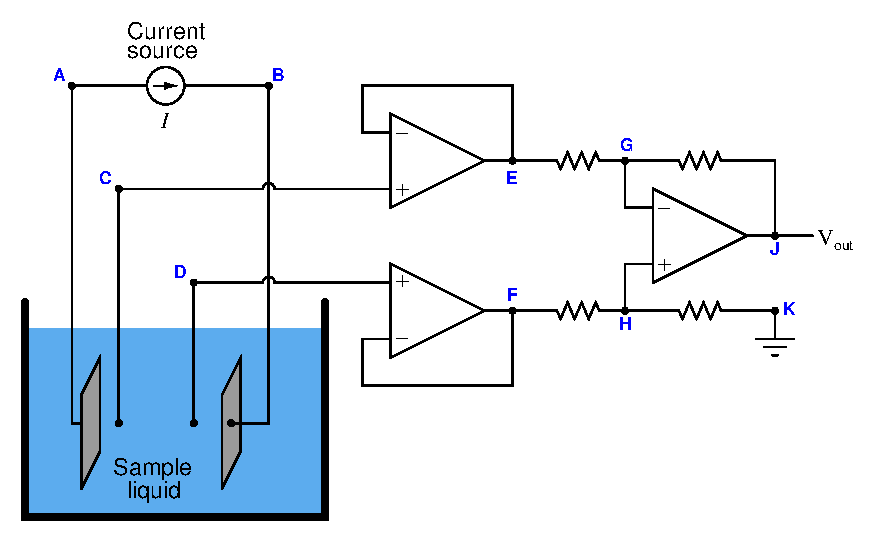
\includegraphics[width=15.5cm]{i00910x02.eps}$$

\vskip 20pt \vbox{\hrule \hbox{\strut \vrule{} {\bf Virtuell feilsøking} \vrule} \hrule}

Denne oppgaven egner seg godt som en ``virtuell feilsøkings''-øvelse. Når du presenterer diagrammet for studentene, forestiller du deg først en bestemt feil i systemet. Deretter presenterer du ett eller flere symptomer på denne feilen (noe som kan observeres av en operatør eller annen bruker). Studentene foreslår så ulike diagnostiske tester for å identifisere feilens art og plassering, som om de var teknikere som feilsøker problemet. Din jobb er å fortelle hva resultatet blir for hver foreslåtte test, og dokumentere resultatene slik at alle studentene ser dem.

Under og etter øvelsen er det nyttig å stille oppfølgingsspørsmål som:

\begin{itemize}
\item{} Hva forteller resultatet av den siste diagnostiske testen om feilen?
\item{} Anta at resultatet av den siste diagnostiske testen hadde vært annerledes. Hva ville det da fortalt om feilen?
\item{} Er den siste diagnostiske testen den beste testen vi kunne gjort?
\item{} Hva ville vært ideell testrekkefølge for å diagnostisere problemet med færrest mulig trinn?
\end{itemize}

%INDEX% Measurement, analytical: conductivity

%(END_NOTES)

